%******************************************************************************%
%                                                                              %
%                                 Interlude                                    %
%                         for Machine Learning module                          %
%                                                                              %
%******************************************************************************%

% =============================== %
\section*{Interlude - To the Multivariate Universe and Beyond!}
% ******************************* %

Until now we've used a very simple hypothesis: $h_{\theta}(x) = \theta_0 + \theta_1 x$.
With this very simple hypothesis we found a way to evaluate and improve our predictions.  

That's all very neat, but we live in a world full of complex phenomena that a model using
this hypothesis would fail miserably at predicting.
If we take weather forecasting for example, how easy do you think it would be to predict tomorrow's temperature with just one variable (say, the current atmospheric pressure)?
A model based on just one variable is too simple to account for the complexity of this phenomenon.

Now what if, on top of the atmospheric pressure, we could take into account the current temperature, humidity, wind, sunlight, and any useful information we can get our hands on?

We'd need a model where more than one variable (or even thousands of variables) are involved.
That's what we call a \textbf{multivariate model}.
And that's today's topic!

% =============================== %
\section*{Interlude - Predict}
% ******************************* %

\begin{figure}[!h]
  \centering
  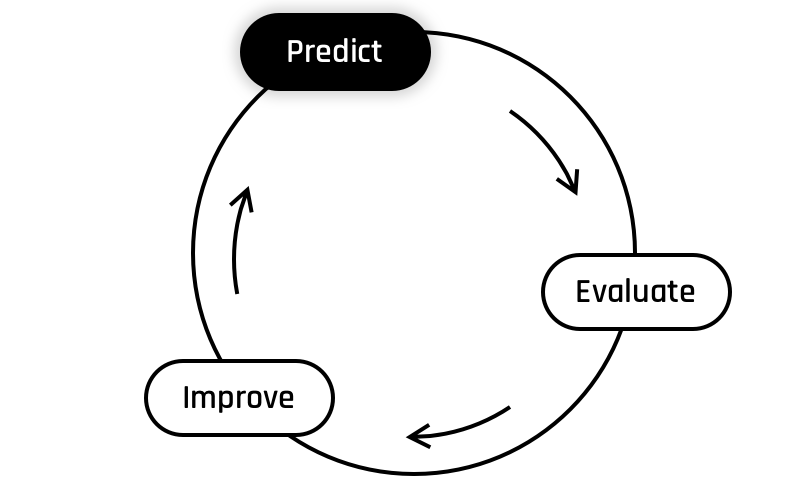
\includegraphics[scale=0.25]{assets/Predict.png}
  %\caption{The Learning Cycle - Predict}
\end{figure}

% =============================== %
\section*{Representing the examples as an $(m \times n)$ matrix}
% ******************************* %
First we need to reconsider how we represent the training examples.
Now that we want to characterize each training example with not just one, but many variables, we need more than a vector. We need a \textit{matrix}!  

So instead of an $x$ vector of dimension $m$, we now have a matrix of dimension $(m \times n)$, where $n$ is the number of \textbf{features} (or variables) that characterize each training example.
We call it the \textbf{design matrix}, denoted by a capital $X$.   

$$
X = \begin{bmatrix} 
x_{1}^{(1)} & \dots & x_{n}^{(1)}\\
\vdots & \ddots & \vdots\\
x_{1}^{(m)} & \dots & x_{n}^{(m)}\end{bmatrix}
$$

Where:
\begin{itemize}
    \item $x^{(i)}$ is the feature vector of the i$^\text{th}$ training example, (i$^\text{th}$ row of the $X$ matrix),
    \item $x_{j}$ is the j$^\text{th}$ column of the $X$ matrix,
    \item $x_{j}^{(i)}$ is the j$^\text{th}$ feature of the i$^\text{th}$ training example (at the intersection of the i$^\text{th}$ row and the j$^\text{th}$ column of the $X$ matrix).
          It's a real number.
\end{itemize}

% =============================== %
\section*{The multivariate hypothesis}
% ******************************* %
Then, we must update our hypothesis to take more than one feature into account. 

$$
\begin{matrix}\large
\hat{y}^{(i)} = \theta_0 + \theta_1 x_{1}^{(i)} + \dots + \theta_n x_{n}^{(i)} & & \text{ for i = 1, ..., m}    
\end{matrix}\normalsize
$$  

Where:
\begin{itemize}
    \item $\hat{y}^{(i)}$ is the model's prediction for the i$^\text{th}$ example,
    \item $x_{1}^{(i)}$ is the first feature of the i$^\text{th}$ example,
    \item $x_{n}^{(i)}$ is the n$^\text{th}$ feature of the i$^\text{th}$ example,
    \item $\theta$ is a vector of dimension $(n + 1)$, the parameter vector.
\end{itemize}

You will notice that we end up with two indices: $i$ and $j$. They should not be confused:
\begin{itemize}
    \item $i$ refers to one of the $m$ examples in the dataset (line number in the $X$ matrix),
    \item $j$ refers to one of the $n$ features that describe each example (column number in the $X$ matrix).
\end{itemize}